\documentclass{book}\usepackage{knitr}

% Preamble

%%%%%%%%%%%%%%%%%%%%%%
%% PACKAGES
%%%%%%%%%%%%%%%%%%%%%%
\usepackage[twoside,letterpaper,width=6in,height=8in]{geometry}
\usepackage{siunitx} % format units properly
\usepackage{wrapfig}
\usepackage[margin=10pt,font=small,labelfont=bf]{caption} % format captions
\usepackage{booktabs} % nicer tables
\usepackage{subcaption} 
\usepackage{csquotes} % block quotes
\usepackage{tikz}
\usepackage[inline, shortlabels]{enumitem} % inline enumeration
%\usepackage[version=4]{mhchem}
\usepackage{graphicx} % packages are used to modify the text and create bling.
%\includegraphics{{Home/CAMPUS/mwl04747/github/Environmnental-Sciences-in-East-Asia/images/}}
\usepackage{textcomp}
\usepackage{gensymb}
\usepackage{natbib}
\usepackage{glossaries}
\usepackage{amsmath}%
\usepackage{amsfonts}%
\usepackage{amssymb}%

%\usepackage[super,square,comma]{natbib}
%\usepackage{float}
%\usepackage{appendix}
%\usepackage{chngcntr}
%\usepackage{etoolbox}
%\usepackage[usenames]{xcolor}% for commenting in color!

\RequirePackage{hyperref} % For hyperlinked cross-references
\hypersetup{
    colorlinks,
    citecolor=blue,
    filecolor=blue,
    linkcolor=blue,
    urlcolor=blue
}


%----------------------------------------------------------
\newtheorem{theorem}{Theorem}
\newtheorem{acknowledgement}[theorem]{Acknowledgement}
\newtheorem{definition}[theorem]{Definition}
\newtheorem{example}[theorem]{Example}
\newtheorem{exercise}[theorem]{Exercise}

\newtheorem{problem}[theorem]{Problem}
\newtheorem{remark}[theorem]{Remark}
\newtheorem{solution}[theorem]{Solution}
\newtheorem{summary}[theorem]{Summary}
\newenvironment{proof}[1][Proof]{\textbf{#1.} }{\ \rule{0.5em}{0.5em}}
%----------------------------------------------------------

\AtBeginEnvironment{subappendices}{%
\chapter*{Appendix}
\addcontentsline{toc}{chapter}{Appendices}
%\counterwithin{figure}{section}
%\counterwithin{table}{section}
}

\makeatletter
\newcommand{\chapterauthor}[1]{%
  {\parindent0pt\vspace*{-25pt}%
  \linespread{1.1}\large\scshape#1%
  \par\nobreak\vspace*{35pt}}
  \@afterheading%
}
\makeatother

\renewcommand{\glstextformat}[1]{\textbf{\color{blue}\em #1}}

\newcommand{\R}{\mathbb{R}}
\newcommand{\carbondioxide}{CO$_2$~}



\title{Environmental Issues in East Asia}
\author{EA30e Spring 2021}
\date{\today}
\IfFileExists{upquote.sty}{\usepackage{upquote}}{}
\begin{document}

\maketitle
\makeglossaries

\frontmatter
\tableofcontents


\chapter*{Preface}

\section{Guiding Principles}

Environmental issues in East Asia are not unique or particularly more prevasive than other parts of the world. However, the issues are born from particular histories that may contrast with other parts of the world and other parts of the world may be able to learn from. 

In this project, the students in EA030e (Spring 2021) have written a textbook that highlights examples of environmental processes. Each student contributed to one theme, composed of two examples that highlight environmental issues of East Asia. 

\subsection{Context and Positionality}

As students in a college course located in Southern California, we approach the project with...


Our goal is not to call out environmental issues in East Asia, but to point to linkages of how a range of globalized economy contribute to these environmental problems. 

In the end, it would be useful for us to acknowledge we have some capacity to address these how these global linkages could be modified to reduce these environmental issues.

We are not experts, but learning... if there are errors please let us know... We recommend that suggestions be submitted via a github pull request.

\subsection{Goals}

Processes across horizontal boundaries define many environmental patterns that frame human interactions with the environment. How do humans impact processes that cross these boundaries and how do humans influence these ecosystem interface?

\subsection{Rationale}

We hope to learn more about the how environmental issues are expressed in different parts of the world and to what extent can we learn from this work. 

\subsection{Activity}

Each group will be composed of two students, that will become experts and teach their classmates on the topic. 

\section{East Asia and the World}







\section{Acknowledgments}

Everyone in the world!




\chapter{\LaTeX Guide}\label{ch:guide}

\subsection*{Why Learn \LaTeX?}

In the past, I used \LaTeX to make publication quality text. In fact, many prefer writing in \LaTeX because they can focus on the text and avoid worrying about formatting. However, it is NOT WYSIWYG (``what you see is what you get'') word processor. In reality, the processing or compiling is a separate step. 

Nevertheless, the quality of the output and ability to integrate with R (or Python) allows us to have an exceptional tool to make reproducible documents. 

\subsection*{How to Learn \LaTeX?}

There are several ways to learn \LaTeX. I suggest you find a decent tutorial to get the basics. For example, here are some suggestions:

\begin{itemize}
  \item \href{https://www.overleaf.com/learn/latex/Learn_LaTeX_in_30_minutes}{Learning \LaTeX in 30 minutes}
\end{itemize}

If you are like me and can't remember commands very well, then here's a \href{https://wch.github.io/latexsheet/latexsheet-0.png}{cheet sheet} that might be helpful. 

\subsubsection{R Chunks}

To create effective graphics, each chapter will have a rchunk that creates a graphic for the chapter. To review and learn R, here are some resources: 

\begin{itemize}
  \item \href{www.tbd.com}{Marc's Video Description}
  \item \href{https://rmd4sci.njtierney.com/}{RMarkdown for Scientists (super helpful!)}
  \item \href{https://rmarkdown.rstudio.com/lesson-1.html}{R Studio Tutorial}
  \item \href{https://rstudio.com/wp-content/uploads/2016/03/rmarkdown-cheatsheet-2.0.pdf?_ga=2.107420162.161662097.1613074083-214354297.1613074083}{R Studio's Cheatsheet}
  \item \href{https://bookdown.org/yihui/rmarkdown-cookbook}{R Markdown Cookbook -- Robust Source}
\end{itemize}


\subsection*{Noting Your Contribution}

Because this is an ongoing project, you should record your contribution to each chapter -- but also let go of these contributions at some point; Others might revise and their authorship might take some precedence, so you should both invest in the product but also be willing to detach from the final outcome as others contribute. This will feel uncomfortable at times, but please note from the beginning this is a social process and as such subject to negotiation. Please be generous to the authors that laid the foundation and be respectful of those that follow. 

\section{Setting Up Book Project--Type Setting w/ \LaTeX}\label{sec:settingup}

\subsection{Latex Book Class}

Currently, the text is written using the standard book class. %However, in 2019, I (Los Huertos) will convert the format to a Tufte book class. 

\subsection{Structuring the Text with Nested Hierarchies}

Contributors divide their contributions into sections and subsections. This format allows a consistent approach to structuring the text and forcing themes to be organized in blocks that can be used to organize the overall text. We use section, subsection, and subsubsection to break up the topic into bite sizes. 

To accomplish this, contributors use the \verb"\section{Section}" command for major sections, and the \verb"\subsection{Subsection}" command for subsections, and a similar approach for subsubsections. 

NOTE: for each nested level, it MUST be followed by the lowest level in the section before a paragraph is started -- in contrast to what is shown above!

NOTE: We may dispense with subsubsections in the future to provide a less blocky structure, but for now they remain useful. 

\subsection{Font Changes}

We can use various methods to alter the typeset: \emph{Emphasize}, \textbf{Bold}, \textit{Italics}, and \textsl{Slanted}. We can also typeset \textrm{Roman}, \textsf{Sans Serif}, \textsc{Small Caps}, and \texttt{Typewriter} texts.  Look online to see the commands to accomplish these changes. 

You can also apply the special, mathematics only commands $\mathbb{BLACKBOARD}$, $\mathbb{BOLD}$, $\mathcal{CALLIGRAPHIC}$, and $\mathfrak{fraktur}$. Note that blackboard bold and calligraphic are correct only when applied to uppercase letters A through Z.

You can apply the size tags -- Format menu, Font size submenu -- {\tiny tiny}, {\scriptsize scriptsize}, {\footnotesize footnotesize}, {\small small}, {\normalsize normalsize}, {\large large}, {\Large Large}, {\LARGE LARGE}, {\huge huge} and {\Huge Huge}.

You can use the \verb"\begin{quote} etc. \end{quote}" environment for typesetting short quotations. Select the text then click on Insert, Quotations, Short Quotations:

\begin{quote}
The buck stops here. \emph{Harry Truman}

Ask not what your country can do for you; ask what you can do for your
country. \emph{John F Kennedy}

I am not a crook. \emph{Richard Nixon}

I did not have sexual relations with that woman, Miss Lewinsky. \emph{Bill Clinton}
\end{quote}

The Quotation environment is used for quotations of more than one paragraph. Following is the beginning of description of \LaTeX from \emph{Wikipedia}:

\begin{quotation}
LaTeX (/ˈlɑːtɛx/ LAH-tekh or /ˈleɪtɛx/ LAY-tekh, often stylized as \LaTeX) is a software system for document preparation. When writing, the writer uses plain text as opposed to the formatted text found in ``What You See Is What You Get'' word processors like Microsoft Word, LibreOffice Writer and Apple Pages. The writer uses markup tagging conventions to define the general structure of a document (such as article, book, and letter), to stylise text throughout a document (such as bold and italics), and to add citations and cross-references. A \TeX distribution such as \TeX Live or MiK\TeX is used to produce an output file (such as PDF or DVI) suitable for printing or digital distribution.

LaTeX is widely used in academia for the communication and publication of scientific documents in many fields, including mathematics, statistics, computer science, engineering, physics, economics, linguistics, quantitative psychology, philosophy, and political science. It also has a prominent role in the preparation and publication of books and articles that contain complex multilingual materials, such as Sanskrit and Greek. \LaTeX uses the TeX typesetting program for formatting its output, and is itself written in the TeX macro language.''
\end{quotation}

Use the Verbatim environment if you want \LaTeX\ to preserve spacing, perhaps when
including a fragment from a program such as:
\begin{verbatim}
#read csv data  // read data into R
my.dataframe <- read.csv(file.choose())   // read data from a popup window.

str(my.dataframe) // display data structure

\end{verbatim}
(After selecting the text click on Insert, Code Environments, Code.)


\subsection{Mathematics and Specialized Characters}\label{sub:mathchar}

\subsubsection*{Warning: Special Characters}

When you use percent and ampersand symbols, hash tags, and other non-standard ASCII characters, \LaTeX will be very uncooperative. \LaTeX~doesn't like a range of characters or they reserved for special behavior. So, do yourself a favor and make sure you understand that these are used for special typesetting functions. To use them you have to ``escape'' and use commands to get them to do what you might usually expect!  

The following symbols \$, \%, \#, \&, \`e, \~n, `` and '' do not reflect the key stroke you might expect. 

For example, the \& is used for tabs in a table environment. \% is used to make comments, thus stuff behind a \% is ignored. There are lots of others, but these come up the most. If you want to show use the ampersand or one of these characters, put a backslash in front of the dollar sybmol, e.g. \textbackslash\$. See Table \ref{tab:tableofsymbols}.

If you want to a superscript (raised to 3nd power), we can create text in math mode, with \$ to start and end the text in math mode, e.g. m$^3$ is written in \LaTeX as m\$\^{}3\$. A subscript uses an underscore, x\$\_1\$ creates x$_1$. If you need more than one character as a subscript or superscript then enclose the content in curly brakets, e.g. x$^{2c}$ (x\$\^{}\{2c\}\$) and t$_{step}$ (t\$\_\{step\}\$).

\begin{table}[h]
\caption{Table of Symbols in \LaTeX}
\label{tab:tableofsymbols}
\begin{tabular}{|ll|ll|} \hline
Symbol  & \LaTeX code & Symbol & \LaTeX code \\ \hline\hline
\&  & \textbackslash\&  & 
\$  & \textbackslash\$ \\
``  & \`{}\`{} & 
''  & \'{}\'{} \\
mg~L$^{-1}$ & mg$\sim${}L\$\^{}\{-1\}\$ & 
    & \\ 
\hline
\end{tabular}

\end{table}

\subsection{Creating equations}

One of the most powerful parts of \LaTeX is how it can be used to write complex equations, with all those symbols and Greek letters! This can be done inline $y = mx + b + \epsilon$ for fairly simple equations, or set apart for more complex equations:

\begin{equation}
\int_0^\infty e^{-x^2} dx=\frac{\sqrt{\pi}}{2}
\end{equation}

\subsubsection{Theorems, etc}
\begin{theorem}
(The Currant minimax principle.) Let $T$ be completely continuous selfadjoint operator
in a Hilbert space $H$. Let $n$ be an arbitrary integer and let $u_1,\ldots,u_{n-1}$ be
an arbitrary system of $n-1$ linearly independent elements of $H$. Denote
\begin{equation}
\max_{\substack{v\in H, v\neq
0\\(v,u_1)=0,\ldots,(v,u_n)=0}}\frac{(Tv,v)}{(v,v)}=m(u_1,\ldots, u_{n-1})
\label{eqn10}
\end{equation}
Then the $n$-th eigenvalue of $T$ is equal to the minimum of these maxima, when
minimizing over all linearly independent systems $u_1,\ldots u_{n-1}$ in $H$,
\begin{equation}
\mu_n = \min_{\substack{u_1,\ldots, u_{n-1}\in H}} m(u_1,\ldots, u_{n-1}) \label{eqn20}
\end{equation}
\end{theorem}
The above equations are automatically numbered as equation (\ref{eqn10}) and
(\ref{eqn20}).


\subsection{Lists Environments: Making bulletted, numbered, description lists}

We use special commands to create an itemized list.

You can create numbered, bulleted, and description lists
(Use the Itemization or Enumeration buttons, or click on the Insert menu
then chose an item from the Enumeration submenu):

\begin{enumerate}
\item List item 1

\item List item 2

\begin{enumerate}
\item A list item under a list item.

\item Just another list item under a list item.

\begin{enumerate}
\item Third level list item under a list item.

\begin{enumerate}
\item Fourth and final level of list items allowed.
\end{enumerate}
\end{enumerate}
\end{enumerate}
\end{enumerate}

\begin{itemize}
\item Bullet item 1

\item Bullet item 2

\begin{itemize}
\item Second level bullet item.

\begin{itemize}
\item Third level bullet item.

\begin{itemize}
\item Fourth (and final) level bullet item.
\end{itemize}
\end{itemize}
\end{itemize}
\end{itemize}

\begin{description}
\item[Description List] Each description list item has a term followed by the
description of that term.

\item[Bunyip] Mythical beast of Australian Aboriginal legends.
\end{description}

\subsection{Theorem-Like Environments}

The following theorem-like environments (in alphabetical order) are available
in this style.

%\begin{acknowledgement}
%This is an acknowledgement
%\end{acknowledgement}

\begin{example}
This is an example
\end{example}

\begin{exercise}
This is an exercise
\end{exercise}


%\begin{proof}
%This is the proof of the lemma.
%\end{proof}

%\begin{notation}
%This is notation
%\end{notation}

%\begin{problem}
%This is a problem
%\end{problem}

%\begin{proposition}
%This is a proposition
%\end{proposition}

%\begin{remark}
%This is a remark
%\end{remark}

%\begin{summary}
%This is a summary
%\end{summary}

\begin{theorem}
This is a theorem
\end{theorem}

%\begin{proof}
%[Proof of the Main Theorem]This is the proof.
%\end{proof}

%\subsubsection{``Child'' Rnw Contributions}

%This is a chapter that we can input into the text... you will each create a chapter without the preamble and begin and end document... that can be integrated into a single book! 

\subsection{Peer Review Commenting}

You can put your comments in square brackets and in color for things that need help. \textcolor{red}{[This section is confusing, I am not sure what commenting means.]}

\subsection{Adding Figures, etc}

\subsubsection{Using Rnw Files}

To generate R figures, we use R chunks in and Rnw file, where the text is integreated. When we compile into a PDF, the program converts the files into TeX files and then combineds them into a single pdf. 

For each chapter, we create a ``child'' document and Marc will help you create that text when you begin. 

\subsubsection{Creating a floating figure}

This is my floating figure (Figure \ref{fig:plot}).

\begin{figure}

\caption{My plot's caption is here!}
\label{fig:plot}
\end{figure}

\subsubsection{Using R to Create Effective Figures}

R Markdown can be a very powerful tool to integrate R code, figures and text. Making high quality figures that are both clear and aestically pleasing will be something that we need to think about it. 

\begin{itemize}
  \item Axis Labels -- Labelled with clarity 
  \item Axis Text -- Size, Orientation 
  \item Captions (usually better than titles)
  \item References connecting labels to references
  \item ADA accessible (e.g. color impairment mitigation)
\end{itemize}

For example, here's code to generate a pretty good figure: 





In the case of Figure~\ref{fig:co2-graphic}, we can a create a figure that has all of the characteristics listed above, except perhaps ADA. Creating a "alt text" for the figure is something we might want to consider -- For now a decent caption about what the reader is seing is super helpful. 

\begin{figure}
\begin{knitrout}
\definecolor{shadecolor}{rgb}{0.969, 0.969, 0.969}\color{fgcolor}
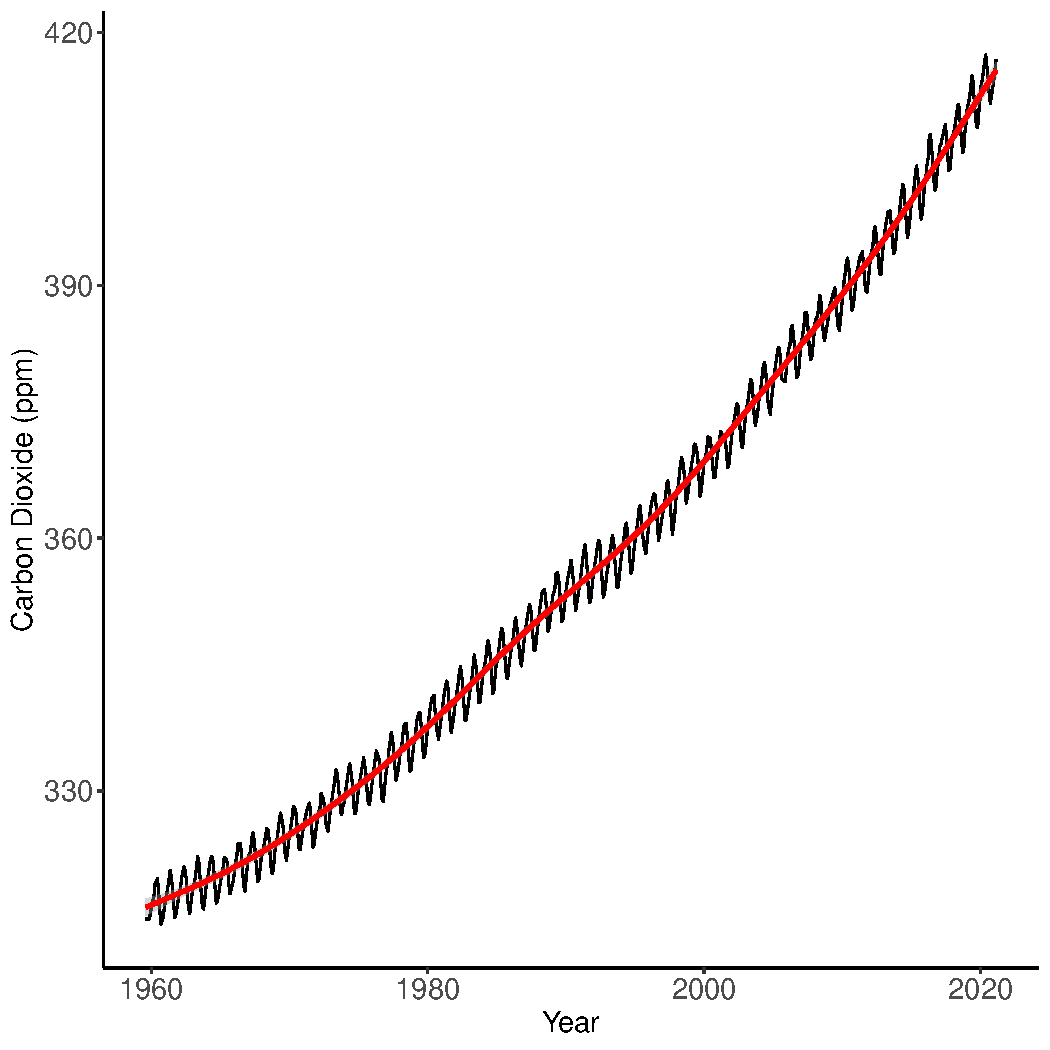
\includegraphics[width=\maxwidth]{figure/maunaloa-1} 

\end{knitrout}
\caption{Carbon Dioxide Concentrations (Mauna Loa, HI). Data demonstrate the CO$2$ concentrations are increases, but that a seasonal impact is embedded in the long-term trend. Source: Scripps/NOAA.}
\label{fig:co2-graphic}
\end{figure}

\subsection{Using Boxes}

\fbox{
\begin{minipage}[c]{.9\textwidth}
\subsection{minibox X}

Some text
\end{minipage}
}

\subsection{Cross-References, Citations, and Glossaries}

\subsubsection{Cross-References}

We can cross-reference sections (e.g. Section~\ref{ch:critical-zone}  or figures (Figure~\ref{fig:maunaloa}) using several methods. I suggest you look at the this Rmd file to see how I did it in these examples.

You can also create links to URLs or hyperlinks, e.g. \url{http://texblog.org}. However, if these addresses change, then the link will break, so I suggest you only link to internal references.

\subsubsection{Bibliography generation}

There will be two steps to cite our sources. First, we need to add the reference to a database, or bib file. This is titled 'References.bib' and is located in the main folder in our respository. When you add information to the bib file, be sure to paste in the reference using a bibTeX format. 

Second, we'll need to place in-line citations, using \verb"\citep{knitr}", which produces \citep{knitr}, by using a key, which is knitr in this case. 

For example, you might write, ``This document was produced in RStudio using the knitr package (\citep{knitr}). Also try \verb"\citet{LosHuertos2017OverviewR}" to create use the author name as the subject: \citet{LosHuertos2017OverviewR} wrote an guide to help students learn R. 

Note: You will see these citations automatically put in alphabetic order in the Bibliography at the end of the PDF. 

%Currently, we are using the ecology.bst, but it has trouble with misc type of references, so I will changing this in 2019. 

\subsubsection{Creating glossary words}
 
\newglossaryentry{peat}{
	name=peat, 
	description={is cool.}
}

\begin{definition}
This is a definition and the word is use in an glossary, e.g. \gls{peat}. \Gls{peat} is when you want to capitalize the defined word without having to re-define a capitalized version, the only downside of case sensitivity in \LaTeX.
\end{definition}


\chapter{Template Chapter Title}\label{ch:template}

\chapterauthor{Chapter Author}

\footnote{Statement of Contributions-- For example, ``The chapter was first drafted by Marc Los Huertos (2021). The author recieved valuable feedback from X, and Y and Z to improve the chapter. Slater revised the chapter in 2022 with suggestions from Cater.'' Note: I am still working on the formatting for this to improve it.}

\section{Section Heading}% Avoid putting text between section and subsection headings.

\subsection{Subsection Headings} % Avoid putting text between subsection and subsubsection headings. Not applicable if you don't have subsections!

Some text here...The hierarchy structure is described in the Author Guide, Section~\ref{sec:settingup} -- NOTE: This is a section cross reference.

if you cut and paste, be sure to make sure you don't include formatted characters outside the ASCII values. See Author Guide, Section~\ref{sub:mathchar}. NOTE: This is a subsection cross reference.


\subsubsection{Optional Subsubsection Headings}\label{subsub:optionalsubsub} % Again try to avoid putting text between the subheadig and the subsubheading to main a structural consistency.

some text here.... and a subsubsection cross reference (See Section \ref{subsub:optionalsubsub}).

\section{Goals of this template}

This template will NOT teach you how to use \LaTeX! To accomplish that, we'll rely on some great online resources that you can find on in Chapter~\ref{ch:guide}. 

Instead this section of the document is designed to demonstrate how our textbook will look, feel, and ultimately how we contribute to the project.

This document also compiles all of our projects into a single PDF, where each chapter is composed of a input tex file.

\section{Here's figure}

\subsection{R Created Figures}

First we create an R chunk and add some code. In this case, I created a floating figure which can be referenced (Figure~\ref{fig:pressure})!  

\begin{figure}
\begin{knitrout}
\definecolor{shadecolor}{rgb}{0.969, 0.969, 0.969}\color{fgcolor}\begin{kframe}
\begin{alltt}
\hlkwd{plot}\hlstd{(pressure)}
\end{alltt}
\end{kframe}
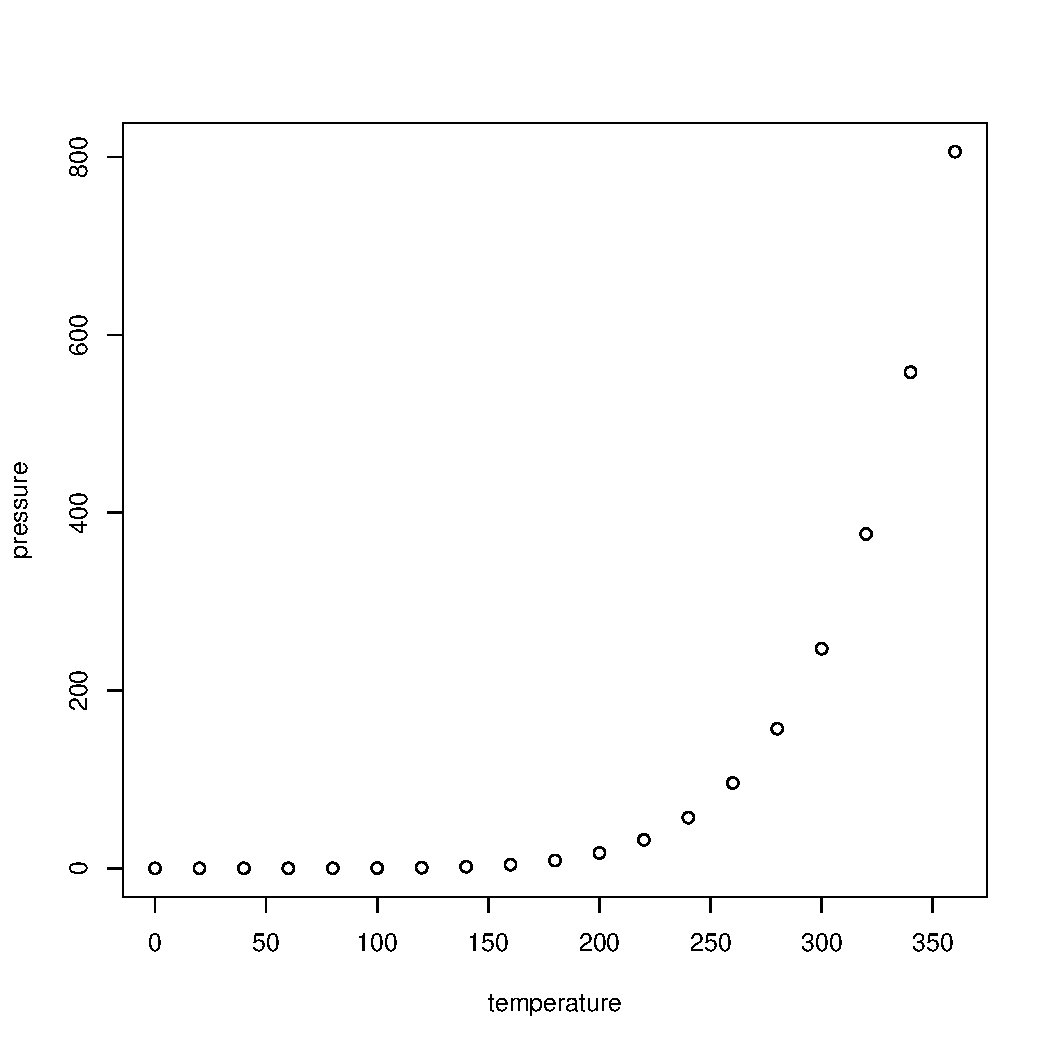
\includegraphics[width=\maxwidth]{figure/fig:pressure-1} 

\end{knitrout}
\caption{Figure Caption...we should turn "echo=False" in the R chunk options, but I left it true for now. (source: ??)} % define the caption, then the label.
\label{fig:pressure}

\end{figure}

\subsection{Floating Figures from External Sources}

All figures and images that are imported should be put into the "images" sudirectory to keep stuff organized. Even better to create a subdirectory with your images, but we can naviagate as we go.

Figure \ref{fig:vadose} is a good example of inserting an image from an external source.

\begin{figure}
\includegraphics[width=\linewidth]{images/Lee-Vadose}
\caption{Vadose zone is neato (Source: \citet{lee2017fifty}).}
\label{fig:vadose}
\end{figure}

In this case, I had to specify the width so it would fit on the page!  See the Rnw file for the code. Notice, I was also abel to ``reference'' the figure in the text.

\section{Adding Citations}

See the Guide, as well, but my video is probably the most helpful.


Generally, there are many environmental trends in Asia \citep{imura2005urban}.

\citet{imura2005urban} describes the how urbanization has affected the hydrology of East Asia. 
 

\chapter{Plastic}

\chapterauthor{Nora}

$\rightarrow$

chekcing on this today, 4-020-2021
pull request test 1.2 

changes at 3 pm, 4-1-21

changes at 3:20 pm, 4-1-21

changes at 3:29 pm 4-1-21



\section{What the Polar Vortex and why do we care?}

test commit and pull request 


\subsection{What Factors Drive Land Use Change?}





\mainmatter


\chapter{The Earth System}\label{earthsystem}

\chapterauthor{Marc Los Huertos}

\section{The Sun's Energy and the Earth's Temperature}

The temperture of the Earth's surface is the result of a balance -- the energy entering the atmosphere and the leaving the atmosphere. Most of this energy is in the form of light or electromagnetic radiation (Figure~\ref{fig:earthbudget}). 

\begin{figure}
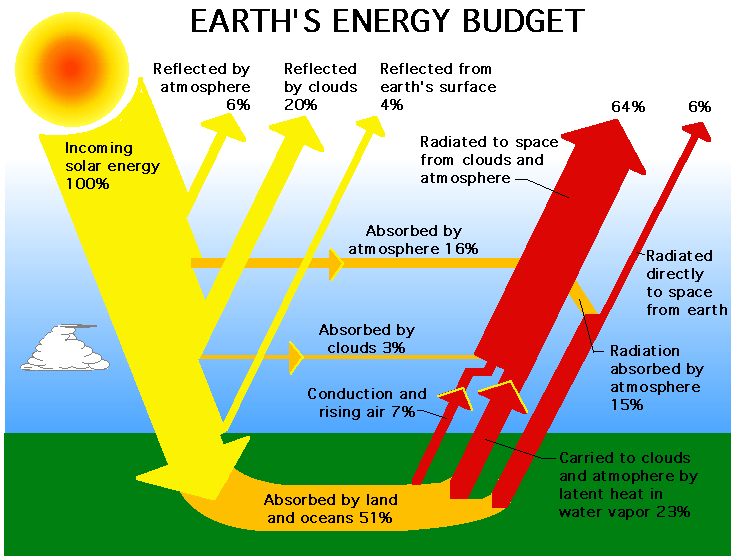
\includegraphics[width=\linewidth]{images/earth-system/earth-rad-budget-nasa-erbe.png}
\caption{caption}
\label{fig:earthbudget}
\end{figure}

Light enters the atmosphere, where some is absorbed and some is reflected. Light interacts in different ways with land, oceans, and vegetation, which is beyond the scope of our project. The ``quality'' of light changes through these processes. 

\subsection{The Spectrum of Light Entering and Exiting the Earth's Surface}

As the sun's electromagnetic radiation interacts with the Earth's Atmosphere, certain wavelengths are absorbed and filtered out (Figure~ \ref{fig:em-entering}).

\begin{figure}
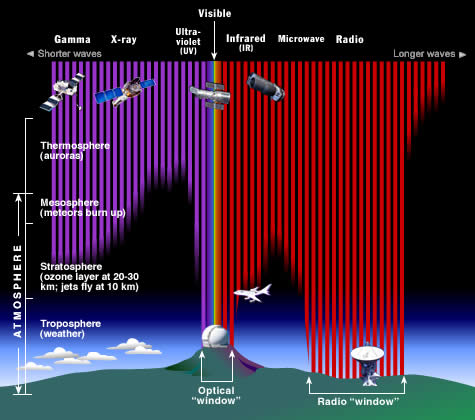
\includegraphics[width=\linewidth]{images/earth-system/em-radiation-atmosph-depth-stsci.jpg}
\caption{Various wavelengths of solar electromagnetic radiation penetrate Earth's atmosphere to various depths. Fortunately for us, all of the high energy X-rays and most UV is filtered out long before it reaches the ground. Much of the infrared radiation is also absorbed by our atmosphere far above our heads. Most radio waves do make it to the ground, along with a narrow `window' of IR, UV, and visible light frequencies. Source: STCI/JHU/NASA.}
\label{fig:em-entering}
\end{figure}

\subsection{The Atmosphere and Greenhouse Effect}



\section{Carbon Biogeochemistry}

\subsection{Long and Short Time Scales}

The carbon cycle processes occur at wide range of temporal scales from hundreds of millions of years to seasons of the year. These have been referred to as long and short carbon cycles. However, for our purposes, I will call them ``geologic carbon'' and ''biosphere carbon'' processes. 

\subsection{Rock Cycle and Geologic Carbon}

The carbon cycle describes changes in the fluxes and reservoirs of carbon in the Earth system. On very long time-scales, millions of years, the primary reservoirs of carbon are the atmosphere, ocean, and rocks (limestone). Carbon moves between these reservoirs through volcanic outgassing, silicate weathering, and limestone sedimentation. The carbon cycle is linked to Earth's energy balance through atmospheric carbon in the form of \carbondioxide, a greenhouse gas.

\subsubsection{Mountains and Erosion}

\ref{fig:carbonpools}

\begin{figure}
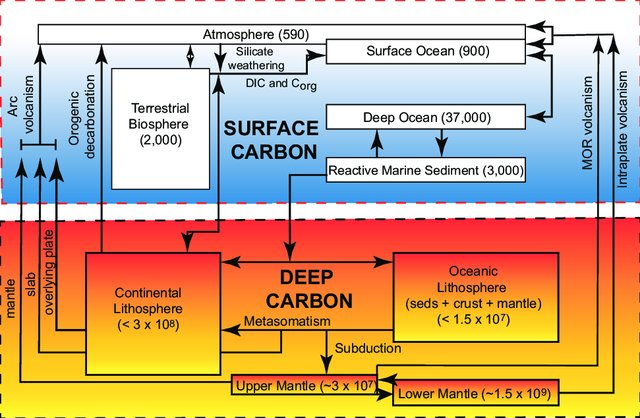
\includegraphics[width=\linewidth]{images/earth-system/Carbon-reservoirs-and-cycles-in-the-Earth.jpg}
\caption{Carbon reservoirs and cycles in the Earth. The figure shows short-and long-term cycles; biosphere and geologic carbon reservoirs and fluxes, and the relative sizes and residence times (y axis) of respective carbon. Numbers in brackets refer to the total mass of carbon in a given reservoir, in Pg C (1Pg C = 10$^{15}$ g carbon). All reservoirs are pre-industrial. Abbreviations: C org = organic carbon; DIC = dissolved inorganic carbon; MOR = mid ocean ridge; seds = sedimentary rocks. Adapted from Lee et al. (2019 And references therein).}
\label{fig:carbonpools}
\end{figure}

\subsubsection{Subduction Burial and Carbon Recycling}

Figure~\ref{fig:longtermcarbon}

\begin{figure}
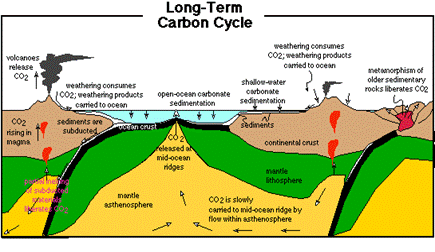
\includegraphics[width=\linewidth]{images/earth-system/long-term-carbon.png}
\caption{Schematic of the long-term carbon cycle (from Bice, 2001)}
\label{longtermcarbon}
\end{figure}

\subsection{Photosynthesis, Respiration, and Biosphere Carbon}

\subsubsection{Soil Respiration and the Soil Profile}

Carbon in soils is respired -- but different pools might have different rates of respiration. Sometimes these pools are distinquished as an active soil organic carbon pool and slow soil organic carbon pool. Although the reference of ``slow'' causes confusion with long-term, geologic carbon, but soil organic carbon remains a component of what we are refering to as biosphere carbon. 

The surface of the soil tends to have more SOC and microbes that can use that carbon for respiration. Lower down in the soil profile, we tend to see lower amounts of SOC and lower microbial biomass (Figure~\ref{fig:soilcarbon}. In addition, soils in the lower part of the profile tend to have more aggregation that protects SOC from microbial attack, thus a key area that soil carbon can seqeustor carbon. 

In addition to these microbial biomass and aggregate patterns, the microbes aree more senstive to temperature changes near the surface as measured by Q10 -- the rate of biochemical processes with a 10 degree C increase in temperature. Thus, soil processes, such as respiration, is likely to increase more near the surface with global warming that the lower part of the soil profile.  

\begin{figure}
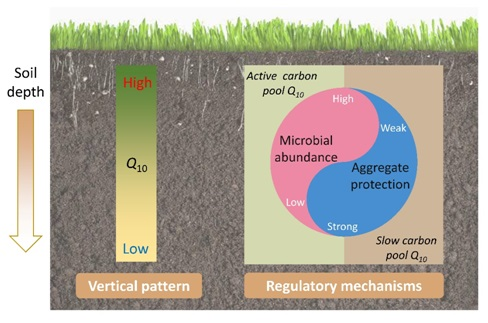
\includegraphics[width=\linewidth]{images/earth-system/Q10-SOC-Regulation.jpg}
\caption{Regulatory Mechanisms of the Temperature Sensitivity of Soil Organic Matter Decomposition in Alpine Grasslands (Source: \citet{Qineaau1218, CAS2021researchers}).}
\label{fig:Q10-SOC}
\end{figure}


\section{Fossil Fuels and Carbon Dioxide Trends}\label{sec:fossilfuels}

As part if the industrial revolution, our energy sources have put more \carbondioxide from the biosphere (soils and forests) and geologic carbon (coal, petroleum). 

\subsection{The Signal of Geologic and Biosphere Carbon in Atmosphere}

The combined contribution from geologic and biosphere carbon in the atmosphere is clearly documented from numerous sources. First, look at data collected at the Mauna Loa where \carbondioxide measurements have been taken continuously since the late 1950s. 

Figure~\ref{fig:maunaloa2}

\begin{figure}
\begin{knitrout}
\definecolor{shadecolor}{rgb}{0.969, 0.969, 0.969}\color{fgcolor}
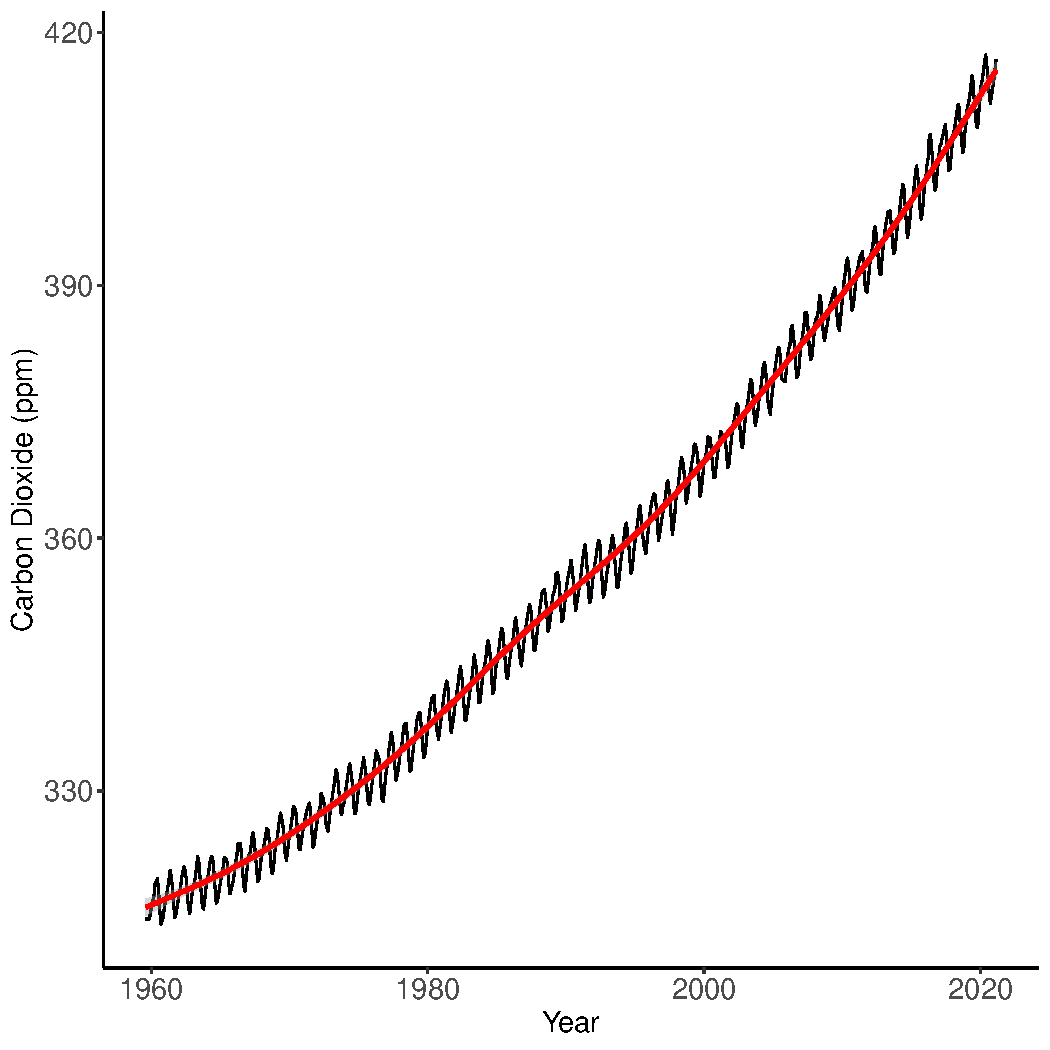
\includegraphics[width=\maxwidth]{figure/maunaloa3-1} 

\end{knitrout}
\caption{Carbon Dioxide Measure on Mauna Loa, HI}
\label{fig:maunaloa2}
\end{figure}






\chapter{Monsoons and East Asia Climates}

\section{Temperature Gradients and Latitude}





\chapter{Critical Zone}\label{ch:critical-zone}

\chapterauthor{Marc Los Huertos}\footnote{The chapter was first drafted by Marc Los Huertos (2021). The author recieved valuable feedback from X, and Y and Z to improve the chapter.}

\section{What is the Critical Zone}

The crticical zone refers the the portion of the Earth's skin where the zone where rock meets life. The Critical Zone supports all terrestrial life.

The critical zone includes the following:

\begin{itemize}
  \item A permeable layer from the tops of the trees to the bottom of the groundwater;
  \item An environment where rock, soil, water, air, and living organisms interact and shape the Earth's surface;
  \item Water and atmospheric gases move through the porous Critical Zone, and living systems thrive in its surface and subsurface environments, shaped over time by biota, geology, and climate.
\end{itemize}

All this activity transforms rock and biomass into the central component of the Critical Zone - soil; it also creates one of the most heterogenous and complex regions on Earth.

Its complex interactions regulate the natural habitat and determine the availability of life-sustaining resources, such as food production and water quality.

These are but two of the many benefits or services provided by the Critical Zone. Such `Critical-Zone Services' expand upon the benefits provided by ecosystems to also include the coupled hydrologic, geochemical, and geomorphic processes that underpin those ecosystems.

\begin{figure}
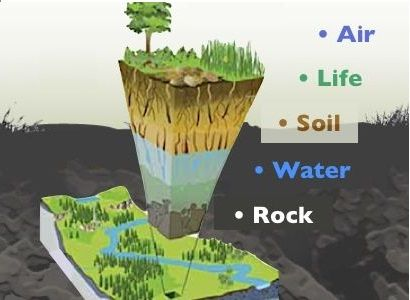
\includegraphics[width=\textwidth]{images/critical-zone/criticalzone.jpg}
\caption{The Critical Zone is an interdisciplinary field of research exploring the interactions among the land surface, vegetation, and water bodies, and extends through the pedosphere, unsaturated vadose zone, and saturated groundwater zone. Critical Zone science is the integration of Earth surface processes (such as landscape evolution, weathering, hydrology, geochemistry, and ecology) at multiple spatial and temporal scales and across anthropogenic gradients. These processes impact mass and energy exchange necessary for biomass productivity, chemical cycling, and water storage.}
\label{fig:criticalzone}
\end{figure}

\subsection{What are the environmental implications of the Critical Zone?}

The critical zone as a concept and as a material space pushes us to think of the porousity of the Earth's surface --- the gas and fluid flows through rocks, soils, and plants. We can begin to appreciate the complexity of the transport and fate of chemical pollutants as they enter the soil and become part of the vadose zone and perhaps the ground water table -- moving with water and diffusing through the water, simultaneously.

\section{Hydrologic Aspects}

\subsection{Subsurface Hydrology}

As water percolates into the soil or flows in the pour space below the surface waters it becomes part of the ground water. The study of this water might be called subsurface hydrology or ground water hydrology or hydrogeology. 

There are two main areas of subsurface waters: saturated zone and unsaturated zone (Figure~\ref{fig:groundwater}).

The saturated zone is the region where all the spaces between the particles are filled by water. The surface of the saturated zone is the water table. 

The unsaturated zone is also called the vadose zone has some percentage of the pour spaces have air. The vadose zone also includes an area called the capillary fringe. Because of the surface tension of water, water is found in between particles above the water table and this zone is referred to as the capillary fringe. 

\begin{figure}
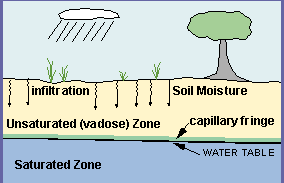
\includegraphics{images/critical-zone/groundwater}
\caption{Diagram of Ground Water. }
\label{fig:groundwater}
\end{figure}

\subsection{Saturated Zone}

\subsubsection{Aquifers and Aquitards}

\subsubsection{Confined and Unconfined Aquifers}

\subsubsection{Ground Water Flow}

TAKE A LOOK at some flow net sketches that will help clarify the relationships between aquifer matrix, and groundwater movement.

In general, water flow is driven by potential energy, e.g.  where water flows down hill, driven by gravity. If water flows from point A to point B, the the potential energy for the flow is the height of the water at point A minus the height at point B, which can be symbolized as $dl$. The head potential is the heigh difference divided by the distance between the two points.  

DARCY'S LAW

\begin{equation}
Q = KIA
\end{equation}

In 1856, Henry Darcy studied the movement of water through porous material. He determined an equation that described groundwater flow. The following description tell how Darcy determined his equation:

A horizontal pipe filled with sand is used to demonstrate Darcy's experiment. Water is applied under pressure through end A, flows through the pipe, and discharges at end B. Water pressure is measured using piezometer tubes (thin vertical pipes installed at each end of the horizontal pipe). The difference in hydraulic head (between points A and B) is dh (change in height). Divide this by the flow length (i.e. the distance between the two tubes), dl, and you get the hydraulic gradient ( I ).

The velocity of groundwater is based on hydraulic conductivity (K), as well as the hydraulic head (I). Therefore, the equation determined by Darcy to describe the basic relationship between subsurface materials and the movement of water through them is Q = KIA where Q is the volumetric flow rate (or discharge) and A is the area that the groundwater is flowing through. This relationship is known as Darcy’s law.

DISCHARGE
%* symbol-Q * units-volume/time EX. (m^3/day) * volume of water flowing through an aquifer per unit time * FIND WITH DARCY'S LAW Q = KIA

AREA OF FLOW
%* symbol-A * units-distance squared EX. (m^2) * Cross-sectional area of flow. (i.e. aquifer width x thickness)

Now, rearrange the equation to Q/A = KI, which is known as the flux (v), which is an apparent velocity. Actual groundwater velocity is lower than that determined by Darcy, and is called Darcy Flux (vx)

FLUX
%* symbol-v * units-distance/time EX. (m/sec) * v=Q/A=KI * this is a velocity measure and gives the IDEAL velocity of groundwater (assumes that the water molecules can flow in a straight line through the subsurface). * this is ideal because it doesn't account for tortuosity of flow paths (this means that the water molecules actually follow a very windy path in an out of the pore spaces and so travel quite a bit slower in reality than the flux would indicate).

DARCY FLUX
%* symbol - vx * units - distance/time EX. (m/sec) * vx = Q/An = KI/n * This is the ACTUAL velocity of qroundwater and DOES account for tortousity of flow paths by including porosity in its calculation.

Darcy's law is used extensively in groundwater studies. It can help answer important questions such as what direction an aquifer pollution plume is moving in, and how fast it is traveling

\subsection{The Vadose Zone}

The vadose zone is the 

Jeji is a volcanic island is located some XX km south of the Korean Penisula. Water runs off the steep slopes quickly and water supplies are limited on the island. To adddress this...\citet{lee2017fifty}.

\begin{figure}
\includegraphics[width=\linewidth]{images/critical-zone/Lee-Vadose.png}
\caption{... (Source: \citep{lee2017fifty}).}
\label{fig:vadose2}
\end{figure}



\chapter{Land Use in East Asia}

chapterauthor{Samantha Beaton}

What is Land Use Change?

What Factors Drive Land Use Change?

How Land Use Change is Measured and Quantified

Integration of sociology

with data science: spatial data compiled from aerial photos, Landsat satellite images, topographic maps, GPS data, etc.

Requires classification and division of land-space types

Ecological Effects of Land Use Change on Soil, Air, and Water

\section{Impacts on Soil}

Deforestation and soil degradation

lack of stability (erosion) and loss of carbon sequestration potential

Forests


coupled with monoculture agriculture

Example Case Study: representative of monoculture agriculture-rice paddies in SE Asia (potentially\ldots)


Impacts on Local Watersheds

hydrology 

infiltration/pollution, groundwater recharge, flow of river basins, runoff

Higher risk of flooding and droughts

\section{Conclusion \& Prospect of Sustainable Urbanization/Land Use Change}


\chapter{Deforestation}\label{ch:deforestation}

\chapterauthor{Xinlan Chen}

\footnote{Statement of Contributions-- For example, ``The chapter was first drafted by Marc Los Huertos (2021). The author recieved valuable feedback from X, and Y and Z to improve the chapter. Slater revised the chapter in 2022 with suggestions from Cater.'' Note: I am still working on the formatting for this to improve it.}

\section{Section Heading}% Avoid putting text between section and subsection headings.

\subsection{Subsection Headings} % Avoid putting text between subsection and subsubsection headings. Not applicable if you don't have subsections!





\section{Overall}
Deforestation is not a small issue in East Asia, since most countries here depend on the money source they got from the wood export industry. There are many issues that could be caused by deforestation with but not limited to air pollution, water pollution and climate change. Upon having looked at all the presentations that people make, I realized that most East Asia countries that was originally covered mostly in forest have significantly reduced in their forest coverage, and nevertheless, natural is punishing them for that. Over-logging is when the level of deforestation exceeds the self-sustaining state of the ecosystem, leading to desertification. Excessive cutting of trees can bring a series of troubles and problems. Many countries have started having regulations on business regarding wood exports and forests protection, more have to be done in order to resolve the issue that people have done in the past that resulted in deforestation. 

\section{Damage Done by Deforestation – Example of China}
After soil erosion and deforestation, the bare land cannot withstand the wind and rain. On sunny days, due to the sun exposure, the ground temperature rises, the process of organic matter decomposition into soluble mineral elements is accelerated; On rainy days, rainwater is washed directly, carrying the fertile topsoil along with mineral elements into rivers. It is estimated that more than 5 billion tons of soil are washed into rivers in China every year. The siltation of quicksand blocked the channel of the reservoir. Sediment concentration in the Yellow River in China is the highest in the world, and when floods come, water and sand are equally divided. Due to the deposition of quicksand, the riverbed in some places in the lower reaches of the Yellow River is 12 meters higher than the land beyond the embankment and even higher than the city wall of Kaifeng City, posing a serious threat to the safety of people's lives and property.
The deteriorate of environment always accompanies with frequent disasters. The forest coverage rate in Wanning County, Hainan Province, used to be as high as 63 percent. Due to forest regulation, there was no drought in the 1940s and 1950s. Since then, natural disasters have been on the rise. From the 1960s to the 1970s, droughts hit an average of six out of every ten years, cutting the flow of 21 rivers, reducing the output of three-quarters of farmland and drying up 25 reservoirs. In particular, the destruction of the forest, so that some rare animals lost their breeding base. Animals there can't survive. China's Hainan slope deer, South China tiger, black - crested gibbon and other precious animals are endangered due to habitat destruction. There is less oxygen supply when deforestation issue is present, consequently there is more carbon dioxide and less natural filters. The ecological environment was forcibly occupied, and the law of ecological circulation was destroyed. The temperature can change, causing unstable changes in the climate.

\section{Overall Losses – Example of Indonesia and Thailand}
In the past decade, Southeast Asia has suffered the greatest loss of forest area, with a net loss of more than 900,000 hectares a year. Trees are widely used as materials in construction, decoration, paper making, metallurgy, chemical industry. Used in paper making, as furniture, chopsticks and other main daily necessities, wood floor, plywood, ceiling and other industrial supplies. Cutting down trees so that people can use the land in their own benefits. To sum up, people cut down trees mainly for their own needs.
	In some parts of Thailand, inspectors inspect thousands of smuggled trucks at roadblocks every day. Instead of guns and drugs, they are carrying wood. Thailand, once a major teak producer in the world, is now on the verge of disappearing its forest resources, and most of the forest areas have become a mess of tree stumps. According to government statistics, Thailand's forest cover has almost halved in two decades. In 1961, it still accounted for 53\% of China's forest areas, and in 1981, it only accounted for 28\%. Some experts believe that the actual forest coverage is much less at present. According to the latest survey report of the United Nations, in South Asia, Southeast Asia and the Pacific Islands, forests are disappearing at the rate of 12500 hectares per day, that is, 4.5 million hectares per year. The report also points out that Indonesia, the largest producer of tropical hardwood in the world, loses more than 1.2 million hectares of forest land every year. Thailand is more serious, with an annual deforestation of 800000 hectares, while the land area of this country is only one fourth that of Indonesia. The large-scale disappearance of forests has caused climate change and the death of wild animals and caused ecological disasters. In Thailand, 42 people died of floods in 1979. If effective measures to protect wildlife areas are not formulated, wild elephants may disappear in 30-40 years. Another reason for the destruction of forests is that mountain tribes in Thailand still carry out primitive farming. They cut down trees to burn wasteland and clear land for farming. According to the United Nations survey, 70\% of the forests in the north have been destroyed. Online Thailand has changed from a major log exporter to an importer, with an annual cost of US \$4400 in foreign exchange.
	Since 1968, Thailand has divided nearly half of the country's forests into more than 500 leased plots for logging. The annual deforestation rate of Southeast Asian countries is relatively high, and the annual reduction of forest area is increasing year by year. Indonesia has increased from 600000 hectares before the 1990s to 1084000 hectares between 1990 and 1995. At the same time, Thailand increased from 244000 ha to 329000 ha, Malaysia from 255000 ha to 400000 ha, Philippines from 91000 ha to 262000 ha, Myanmar from 102000 ha to 387000 ha. Compared with the period before the 1990s, the annual average amount of logging in these countries increased by one cup in the first half of the 1990s, and even tripled in some countries. Since Vietnam's reform and opening up, due to a large number of logging and fire, the forest area has also been greatly reduced. From 1990 to 1995, a total of 1.5 million hectares of forest were lost, that is, 26000 hectares per year. In recent years, four of the six countries with the most deforestation in the world are Southeast Asian countries. Their average annual felling rates are 513300 acres in Thailand, 400500 acres in Myanmar, 396000 acres in Malaysia and 316100 acres in the Philippines. From 1969 to 193, about 6000 square kilometers of forests, swamps and grasslands were opened up for agricultural use by immigrants in Indonesia. Although forest is a renewable resource, its growth cycle is decades or even hundreds of years. For a long time, a large number of forests have been cut down in Southeast Asia, but the work of forest restoration and afforestation has not been given due attention. The speed of forest restoration is far behind the speed of deforestation, resulting in the decrease of forest area year by year.

\section{Correlation Between Deforestation and Pandemic}
Deforestation has led to more outbreaks of human infectious diseases, and in 1997, in Indonesia, a haze shrouded the rainforests, an area the size of Pennsylvania was burned to promote agriculture, and droughts exacerbated the fires. Under the smog, the trees are unable to bear fruit, leaving local fruit bats with no choice but to fly elsewhere in search of food, and carry with them a deadly disease. Soon after the bats took up residence in the trees in the Malaysian orchards, nearby pigs began to get sick -- probably from eating fallen fruit eaten by the bats, and local pig farmers also began to get sick. By 1999, 265 people had severe encephalitis and 105 had died. This was the first known case of Nipah virus in humans, and since then there have been a series of repeated outbreaks across Southeast Asia. Such infectious diseases are usually confined to wild animals but are spreading to areas where forests are being cleared rapidly. Human infections vary from asymptomatic to fatal encephalitis. Infected people initially develop flu-like symptoms: fever, headache, muscle pain, vomiting and sore throat. This may be followed by dizziness, lethargy, confusion, and neurological signs that indicate acute encephalitis. Some people may also develop atypical pneumonia and serious respiratory problems, including acute respiratory distress. In severe cases, encephalitis and epilepsy develop, leading to coma within 24 to 48 hours. The time between infection and onset of symptoms ranges from four to 45 days. Most acute encephalitis survivors who recovered from it are left with residual neurological consequences, such as persistent seizures and personality changes. A small number of people recover and relapse or develop delayed encephalitis. Over the long term, persistent neurological dysfunction has been observed in more than 15\% of the population. The case mortality rate is estimated at 40\% to 75\%. Over the past two decades, scientific evidence has mounted that deforestation sets off a complex chain reaction that sets the stage for a host of deadly pathogens to spread to humans, like Nipah and Lassa viruses, as well as the parasites that cause malaria and Lyme disease. Today, large areas of the Amazon rainforest, parts of Africa and Southeast Asia are still burning, and experts are concerned about the health of people living on the edge of deforestation. They also worry that the next serious pandemic could emerge from the planet's forests. Researchers have identified the correlation between malaria and deforestation, which kills more than a million people a year and is mainly transmitted by the malaria parasite carried by mosquitoes.

\section{Data Proving the Damage of Deforestation as a Broader Picture and Policy Implemented}
In Southeast Asia, the area of forest is gradually decreasing, and the forest coverage rate is decreasing due to the migration and reclamation, deforestation, expansion of farmland, backward farming methods and large-scale commercial forest development. Before the 1970s, the forest coverage rate of Indonesia, Cambodia, Laos and Brunei was as high as 70\%, that of Myanmar and Malaysia was 66\%, and that of Vietnam, Philippines and Thailand was less than 50\%. By 1995, the forest coverage of these countries had decreased significantly, to 55.7\% in Cambodia, 41.3\% in Myanmar and 47.7\% in Malaysia. 60.6\% in Indonesia, 22.8\% in Thailand and 22.7\% in the Philippines. Forest is the habitat of animals. With the decrease of forest area, the habitat of animals and plants also decreases.
	The rate of net loss is significantly lower than the annual loss of 2.4 million hectares during the period 1990-2000. Despite a net increase in forest area reported at the regional level, the rate of deforestation remains high in many countries. In the past decade, Southeast Asia has suffered the greatest loss of forest area, with a net loss of more than 900,000 hectares a year. However, the rate of net loss is significantly lower than the annual loss of 2.4 million hectares during the period 1990-2000. Overall, the Asia and Pacific region lost 700,000 hectares of forest per year in the 1990s but gained 1.4 million hectares per year between 2000 and 2010. This is largely the result of China's massive reforestation efforts, which saw the country's forest area increase by 2 million hectares a year in the 1990s and an average increase of 3 million hectares a year since 2000. As article 8 of the Forest Law of the People's Republic of China stipulates that the state shall implement the following protective measures for forest resources: (1) implement quota cutting for forests, encourage afforestation, close mountains for forest cultivation, and expand the area covered by forests; (2) to give economic support or long-term loans to collectives and individuals for afforestation and forest cultivation in accordance with the relevant provisions of the state and local people's governments; (3) To advocate the comprehensive utilization and economical use of wood and encourage the development and utilization of wood substitutes; (4) Collect forest raising fees and use them exclusively for afforestation and forest raising; (5) In the departments of coal and paper making, a certain amount of funds shall be set aside according to the output of coal, wood pulp and paper to be used exclusively for the construction of pit timber and timber for paper making; (6) Establishing a forestry fund system. The State shall establish a forest ecological benefit compensation fund to be used for the construction, upbringing, protection and management of protection forests that provide ecological benefits and forest resources and trees with special uses. Forest ecological benefit compensation funds must be earmarked for special purposes and may not be misused for other purposes. Specific measures shall be formulated by the State Council. Bhutan, India, the Philippines and Vietnam also reported an increase in forest cover over the past 10 years. Despite a net increase in forest area reported at the regional level, the rate of deforestation remains high in many countries. In the past decade, Southeast Asia has suffered the greatest loss of forest area, with a net loss of more than 900,000 hectares a year. China, India and Vietnam have all set targets for large-scale reforestation, as well as incentive programs to encourage small farmers to plant more trees. China plans to increase its plantation area by 50 million hectares to 23 percent by 2020. If the current rate of afforestation continues, it may be possible to achieve this goal by 2015. India has set a goal of 33 percent forest and tree cover by 2012. Forests, other woodlands or land covered with trees accounted for about 25 percent of India's land area in 2010, according to the Global Forest Resources Assessment. The area of unknown rows of trees planted and other "trees outside the forest" should be included in this percentage. The government's goal was to restore forest cover to 43 per cent by 2010, and according to information provided to the Global Forest Resources Assessment, this goal has been met.

\section{Suggestions}
(1) Strengthening the awareness of forest resources protection
The human living environment is increasingly bad, the ecological environment problem has become the focus of globalization. The destruction of forest resources leads to soil erosion, land desertification, poor air quality and even harm to human health. We should realize the importance of forest resources, strengthen the awareness of forest resources protection, the protection of forest resources is everyone's responsibility, starting from ourselves, fundamentally accept and support the forest resources protection policy, dare to report illegal logging behavior, participate in the protection of wild animals and plants. On the basis of not destroying, afforestation can promote the healthy and sustainable development of forestry, mobilize the enthusiasm of the broad masses of people, effectively protect forest resources to the greatest extent, improve the ecological environment, and enable people to live in harmony with nature.
(2) Strengthening the construction of forest resources management institutions
The management and protection of forest resources should be based on the principle of sustainable development and operation, and rational harvesting should be carried out according to the quality and structure of forest resources. Forest resources management agencies should be established and the management system should be improved. According to the actual situation of forest resources, forest management and protection stations should be set up reasonably, and the management and protection personnel should be trained to improve their management and protection ability and legal awareness of forest resources. We should reasonably formulate quotas for forest cutting, conduct management and supervision over the issuance of cutting licenses in accordance with the Forest Law, ensure that there are laws to follow for cutting with vouchers, supervise the progress and management of cutting, and resolutely prohibit arbitrary cutting. Forestry departments should also adapt to the requirements of the current social development situation, under the trend of rapid development of information, increase investment to improve hardware and software infrastructure, establish a perfect information system, improve configuration facilities, improve work efficiency. The perfect forest resources information management system, standardized management data collection and analysis, improve the level and quality of monitoring, scientific management and protection of forest resources.
(3) Strengthening control of diseases and insect pests of trees and protection against forest fires
Natural disasters of forest resources mainly have two aspects, one is pests and diseases, the other is forest fires. These two kinds of harm to the forest destruction and loss are huge. As for the prevention and control of diseases and insect pests, the quarantine of quarantine forest plants and the prevention and control of forest diseases and insect pests should be strengthened. The Quarantine Law should be strictly implemented to prevent the introduction of harmful organisms and put an end to the man-made spread of pests. Monitoring and forecasting of forest diseases and insect pests, taking the initiative to prevent disasters and effectively control the scope and harm of diseases and insect pests; On the other hand, the prevention and control of forest fires has always been the top priority of forest resource management. For a long time, the need to constantly, vigorously adhere to the propaganda of fire prevention work, multimedia, multi-faceted personnel into the forest to strengthen the awareness of fire prevention, has been unable to relax vigilance. Implement the fire prevention responsibility of relevant units, control fire source management, carry out regular joint prevention of responsible households, establish and perfect fire monitoring and forecast system, strengthen the allocation of fire prevention equipment, fundamentally control fire sources, timely control when fire occurs, and reduce the loss of forest resources.
(4) Improve the utilization rate of forest resources
The utilization of forest resources is mainly the development of forestry, and the industrialization of forestry development is its development trend. In the management and management of forestry, we should first cultivate forest resources fundamentally, increase the intensity of forest cultivation, improve the quality of forest resources and improve the ecological environment. On this basis, forestry industrialization, technological production technology improvement, research and development of new wood processing industry, adjust the direction and structure of wood products. At the same time, the comprehensive development of forest resources, the development of breeding, planting, and related processing industries, in many ways to improve the maximum utilization rate of forest resources.


\chapter{Invasive Species}

\chapterauthor{Soliel}

\footnote{Statement of Contributions-- For example, ``The chapter was first drafted by Marc Los Huertos (2021). The author recieved valuable feedback from X, and Y and Z to improve the chapter. Slater revised the chapter in 2022 with suggestions from Cater.'' Note: I am still working on the formatting for this to improve it.}

\section{Section Heading}% Avoid putting text between section and subsection headings.



\chapter{Nuclear Power and Nuclear Waste}

\section{Current and Future Energy Needs}



\chapter{Air Pollution \& Social Justice in Hong Kong}

\chapterauthor{Neenah Vittum}

\section{Science of Air Pollution}

\subsection{Overview of the layers of the atmosphere/atmospheric gases}

What part of the atmosphere does air pollution affect?

What is air pollution?

Overview of different types of air pollution

\section{Major Sources → Use as geographical overview}

\subsection{General common sources of air pollution all over the world}

\subsection{East Asian countries/communities and their prominent air pollution sources}

Shipping

Traffic Emissions

Commercial and otherwise

Coal

Urban Development

Manufacturing

Other

The transboundary issue and its implications in regulation and politics

Impacts

Human health

Environmental Health

Greenhouse gas emissions and global warming

Both

Visibility

Environmental Justice

Case Study: Hong Kong

The Intersection of Air Pollution and Other Environmental Issues

Many environmental issues are interconnected

Air pollution and deforestation

Air pollution and urbanization/industrialization

Other Issues (To Explore)

Goals/Other Ideas/Questions

Ground information in geography and relevant examples

Incorporate stories and person accounts

slow violence → environmental justice issues

Maybe activist or someone who has suffered the issues firsthand

Draw people into the empathy

Use stories and descriptions to describe places

What is the best way to section the chapter?


\chapter{Flood Pulse System in East Asia}

\chapterauthor{Kristin Gabriel}

\section{Introduction}

What is the flood pulse system?

Seasonality

Ecosystem Services

Fish stocks

Flooded forests

How the flood pulse system influences the Tonle Sap Ecosystem

Timing of Flood Pulse

Magnitude of Flood Pulse

Duration of Flood Pulse

Influence of flood pulse system on people and their livelihoods

Fisheries

Immigration and emigration

Human Impacts on the flood pulse system

Climate change

Dam development

Case Study: Cambodia and the Tonle Sap


\chapter{Hydroelectric Dams in East Asia}

\section{Introduction}

Basic facts about dams in East Asia


Statistics on how many, size, scale, location etc.

Function of the Dam 

How it generates electricity/how much

Different types of dams (multi/single use etc.) 

Immediate ecological impacts 

Positive: 

Flood control, electricity generation, improved water quality 

Negative: 

Decreased water quality, flooding, sedimentation, habitat loss, deforestation, salinization etc... *note: the ecological impacts may be too many to go completely in depth into so perhaps a paragraph or subsection of each as opposed to a 7 page explanation of each 

Anthropological impacts 

Supposedly positive (I.e. employment etc...)

Negative: displacement, loss of cultural sites, diseases 

Displacement

Policy/government action/regulation  (policies that exist or propose solutions)

\section{Conclusion}



\chapter{Climate Change and Food Security in Myanmar}



\section{Climate Change, Climate Change Response in Myanmar}


General history of rice production and food demand in Myanmar. 

Impact on credit policy on rice 

Impact of infrastructure development on rice production

Study of the constraints of rice production in Myanmar

The effect of a command economy on food production in Myanmar 

Overall review on demand for food in Myanmar 

Possible implementation of SRI (systemic rice intensification) in order to increase rice yields in Myanmar

Transition from talking about rice production

sea-level rise

subsidence

coastal erosion

coastal flooding

Impact of climate change on rice production in Southeast Asia

Monsoon Season effect on Ayeyarwady River Badin

Sea Level Rise 

Sea level rise effect on global markets/rice production


Subsidence

Subsidence in Yangon, Myanmar

interview segments/personal experiences of rice farmers


Roles of the Burmese government

\section{Conclusion}

Reminders/Areas of Focus




\chapter{Disasters, Typhoons and Phillipines}

\chapterauthor{Ian Horsburgh}

\section{What are Typhoons?}



\chapter{Climate Infrastructure in Vietnam}

\section{Introductory}

How climate change will impact Vietnam

Flooding (especially coastal urban areas)

Sea Level Rise

Land Erosion

Health outcomes

Current Adaptation Plans

Strengthen existing barriers and infrastructure

Adapt cities expecting sea level rise

Withdraw from the coastlines in areas that are well below sea level

What's Needed for the Future

Stronger healthcare system

Support for farmers and agricultural workers

Support for rural population near Mekong and Red river deltas

\section{Conclusion}

Implications for other places in the region


\chapter{Waste Management for a Circular Economy}

\section{Life-Cycle}

\subsection{Collection}

\subsection{Transport}

Treatment

Disposal

Sectors:

Industrial

Household

Biological 

Types of Waste:

Solid:

Liquid

Gaseous waste

\section{Biomimicry}

\subsection{Circularity}

Examples in Nature

Education:

Teach people to be mindful and live sustainably

Social PsychologyProblems and New Approaches: 

Sustainability

Incineration \& Dumping

Recycle \& Reuse

Resource Recovery


\chapter{Plastic and Packaging in Japan}

\section{Introductiona and Goals?}

Plan: Use Japan's unique plastic packaging as a lens to view plastic waste management. I can bring in benefits of their plastic use, like cultural significance of beautiful wrapping and food safety, and then discuss plastic pollution as a larger issue in East Asia, bringing in examples of blame placing, and of course discussing potential solutions on both international and local scales. 

\section{Plastic Pollution and Waste Management in East Asia} 

\subsection{Statistics/comparisons}

graphs and images will help with perspective

\subsection{History of plastic waste issues in East Asia}

\subsubsection{Are specific companies/industries responsible responsible}

what kinds of plastic waste are there (sector break down)? 

\subsubsection{Where in the world did the ubiquitous usage of single use plastics come from?}

General blame placing/biases/rhetorical 

examples of discourse around plastic waste in East Asia. Why does any of this matter(needs its own section)?

Plastic waste trade? 

\url{https://link.springer.com/article/10.1007%2Fs10163-004-0115-0}

\url{https://www.sciencedirect.com/science/article/abs/pii/S0956053X20305602}

Blame placing through both rhetoric and scientific studies

(this source is a very data based study that concluded that the vast majority of plastic pollution comes from a few sources in Asia/Africa... I want to explore what they might not have taken into account when collecting data)

\url{https://science.sciencemag.org/content/347/6223/768}

\url{https://pubs.acs.org/doi/10.1021/acs.est.7b02368}

\url{https://www.dw.com/en/whose-fault-is-plastic-waste-in-the-ocean/a-49745660} (found the two above studies through this article)

Japan Specific (I need to break these into hierarchies of significance), some sections, the first  few will be more data based, the second half will be more rooted in sociological primary sources.

Waste management issue overview

Sector Break Down/ responsible parties in Japan

Impacts of plastic pollution on different groups within Japan

Cultural significance of wrapping

Food safety

Gov action/recycling/current efforts

Activism

Potential solutions moving forward rooted in current activist efforts/respect to culture

\url{https://www.pnas.org/content/117/33/19844.short}

\url{https://www.jstor.org/stable/432317?seq=1}

\url{https://onlinelibrary.wiley.com/doi/abs/10.1002/1099-1522(200003/04)13:2%3C45::AID-PTS496%3E3.0.CO;2-%23}






\backmatter

\part{Backmatter}

The back matter often includes one or more of an index, an afterword, acknowledgments, a bibliography, a colophon, or any other similar item. In the back matter, chapters do not produce a chapter number, but they are entered in the table of contents. If you are not using anything in the back matter, you can delete the back matter TeX field and everything that follows it.

\printglossary

\renewcommand\bibname{References}
\setlength{\bibsep}{2\baselineskip}
\setlength\bibindent{.5in}
\bibliographystyle{plainnat}
\bibliography{References}

\end{document}
